\usetikzlibrary{arrows.meta}
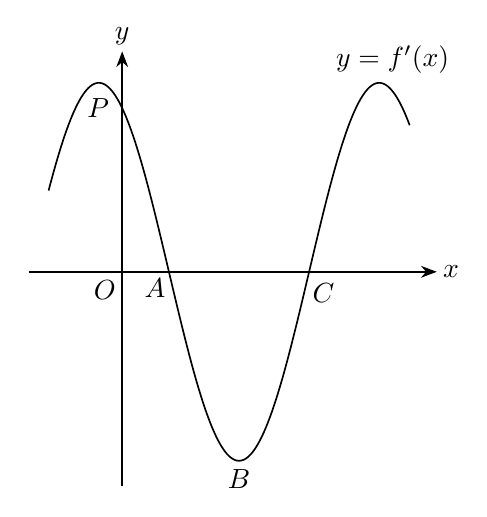
\begin{tikzpicture}[x=1.7cm,y=0.8cm,line width=.6pt,>=Stealth,font=\normalsize]
\coordinate (O) at (0,0);
\coordinate (P) at (0,2.598076);
\coordinate (A) at (0.349066,0);
\coordinate (B) at (0.872665,-3);
\coordinate (C) at (1.396263,0);
\draw[->] (-0.7,0)--(2.35,0) node[right,inner sep=0pt,xshift=2pt] {$x$};
\draw[->] (0,-3.4)--(0,3.5) node[above,inner sep=0pt,yshift=2pt] {$y$};
\draw[domain=-0.55:2.15,samples=201] plot (\x,{3*cos(deg(3*\x+pi/6))});
\node[inner sep=0pt] at (-0.18,2.6) {$P$};
\node[below left,inner sep=0pt,xshift=-1pt,yshift=-2pt] at (A) {$A$};
\node[below right,inner sep=0pt,xshift=1pt,yshift=-4pt] at (C) {$C$};
\node[below,inner sep=0pt,yshift=-3pt] at (B) {$B$};
\node[below left,inner sep=0pt,xshift=-2pt,yshift=-3pt] at (O) {$O$};
\node[above right,inner sep=0pt,xshift=2pt,yshift=2pt] at (1.55,3.05) {$y=f'(x)$};
\end{tikzpicture}
